\documentclass[graphics]{beamer}

\usepackage{graphicx}
\usepackage{verbatim}
\usepackage{wrapfig}
\useoutertheme{shadow}
%\usecolortheme{orchid}
\usecolortheme{seahorse}


% math commands
\newcommand{\be}{\begin{eqnarray}}
\newcommand{\ee}{\end{eqnarray}}
\newcommand{\beq}{\begin{equation}}
\newcommand{\eeq}{\end{equation}}
\def\simless{\mathbin{\lower 3pt\hbox
      {$\rlap{\raise 5pt\hbox{$\char'074$}}\mathchar"7218$}}}
\def\simgreat{\mathbin{\lower 3pt\hbox
      {$\rlap{\raise 5pt\hbox{$\char'076$}}\mathchar"7218$}}} %> or of order

% variables

\def\toonscale{0.45}
\def\mboxy#1{\mbox{\small #1}}


\begin{comment}
\AtBeginSection[]{
  \frame{
    \frametitle{Outline}
    \tableofcontents[currentsection]
  }
}
\end{comment}

\title{Cosmological Wave Optics
}
%\subtitle{interim update}
\author[U. Pen]{Ue-Li Pen
}
\date{January 24, 2021}


\begin{document}

%\section*{Introduction}
\section{Lenses}

\begin{comment}
  \subsection{Outline}

  \frame{
    \frametitle{Outline}
    \tableofcontents
  }
\end{comment}

\frame{\maketitle}



  \frame{
    \frametitle{Coherent Light Sources}
    \begin{itemize}
    \item coherent sources: GWs, pulsars, FRB
    \item not geometric optics
    \item everything is an interference (speckle) pattern
    \item interference pattern between multiple paths      
    \item low dimensionality
    \item alternative picture for quantization: quantum gravity?
    \end{itemize}
  }


  

  \frame{
\vspace{-0.25in}
    \frametitle{Scintillation Holography: Walker 08}
%\begin{center}
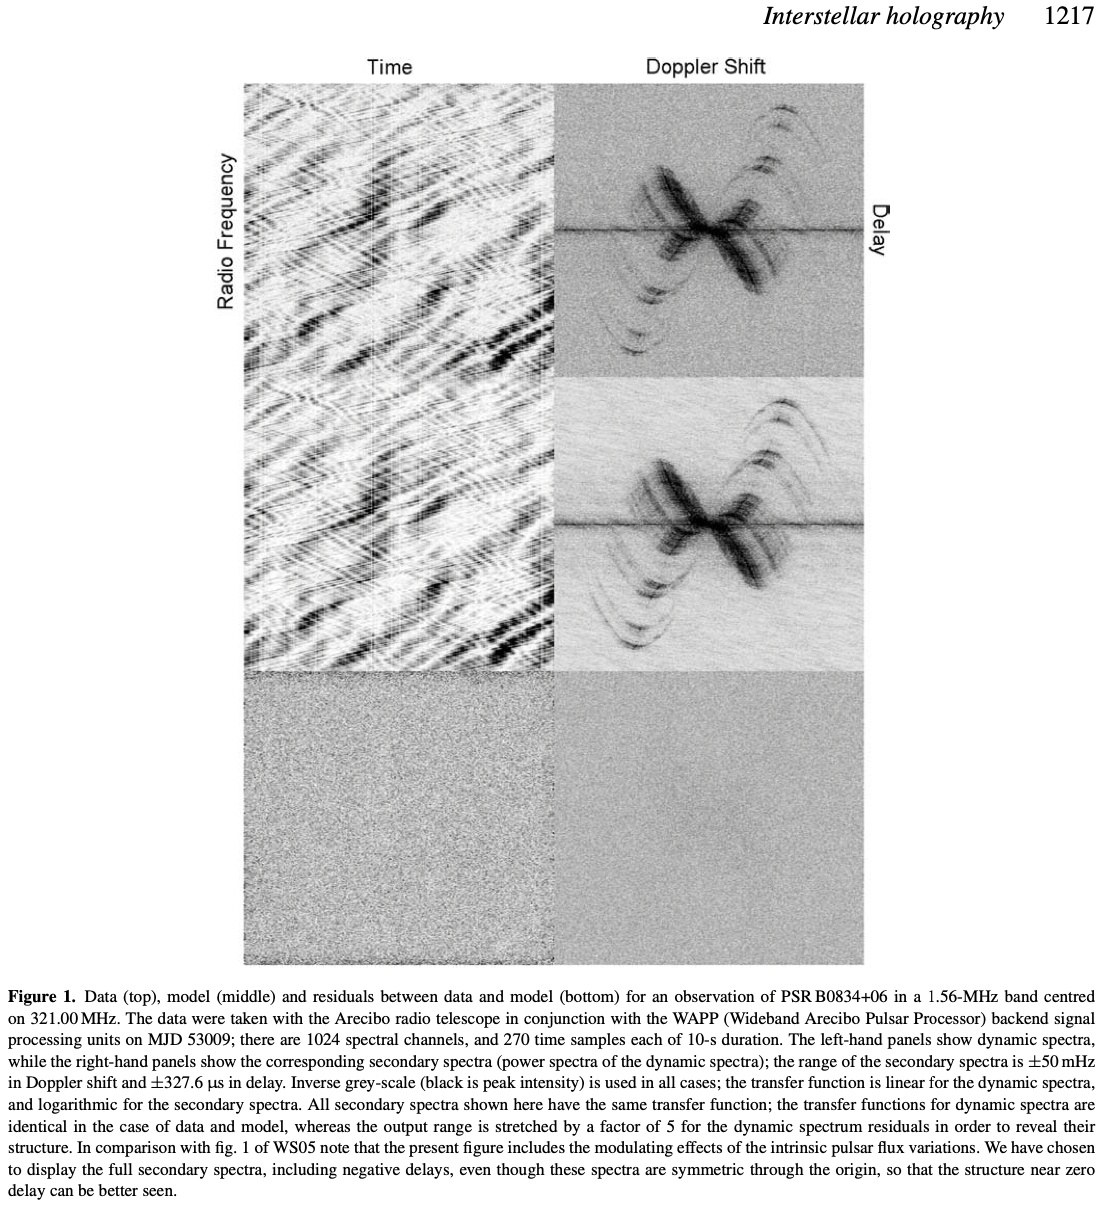
\includegraphics[width=2.51in]{Figures/walker08.png}
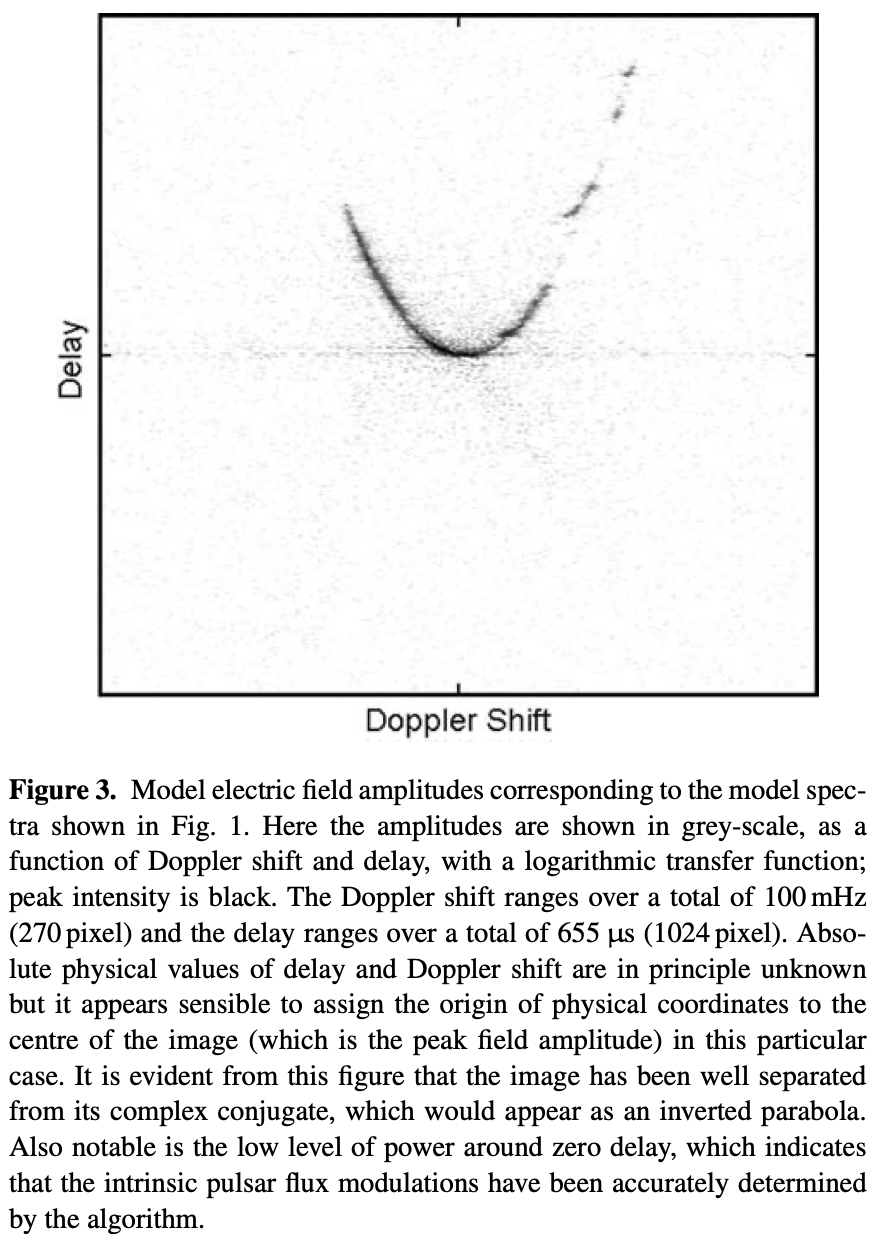
\includegraphics[width=1.9in]{Figures/walker2.png}
%\end{center}
  }





  \frame{
\vspace{-0.5in}
    \frametitle{New Observables}
    \begin{itemize}
    \item for coherent sources: FRBs, pulsars
    \item microlensing: instant time delay, planets (Jow+20)
    \item macrolensing: potentially nano-second delay -- universe
      expands!  Dark energy, etc (Wucknitz+21)
    \item dimensionless strain cm/Gigalightyears $h\sim \Delta t/t \sim 10^{-26}$:
      competitive with LIGO, etc
    \item weak lensing: imaginary image allows time delay measurement (Jow+21)
    \item strong lensing: delay measurements enable measurement of
      co-linearity (Jow++21)
    \end{itemize}
  }


  \frame{
\vspace{-0.5in}
    \frametitle{Macrolensing}
    \begin{itemize}
    \item Wucknitz+ 2021
    \item alternate approach to cosmography
    \item triangulation: lens model+time delay measurement = $H_0$
    \item weak link has been lens model
    \item Wave optics: time delay observable to nanoseconds
    \item For repeating FRB, dominated by galaxy transverse
      motion. then cosmic expansion
    \item individual macrolens images split into microlens images by stars
    \end{itemize}
  }



  \frame{
\vspace{-0.5in}
    \frametitle{Discussion}
    \begin{itemize}
    \item Eikonal effects applicable to compact radio sources,
      e.g. FRBs, pulsars
    \item full wave
effect dominates for long wavelengths as Fresnel scale is bigger then Einstein radius
    \item down to planet size
    \item gravitational waves:  LIGO, LISA, PTA
    \end{itemize}
  }



  \frame{
\vspace{-0.5in}
    \frametitle{Current status}
    \begin{itemize}
    \item Eikonal: pulsar scintillation, wind magnification (Main+ 2018)
    \item full wave optics: pulsar wind lensing, solar wind (IPS)
    \item quantum cosmology, quantum gravity: Feldbrugge++ 
    \end{itemize}
  }

\frame{
    \frametitle{Microscope}
     \vspace{-0.65in}
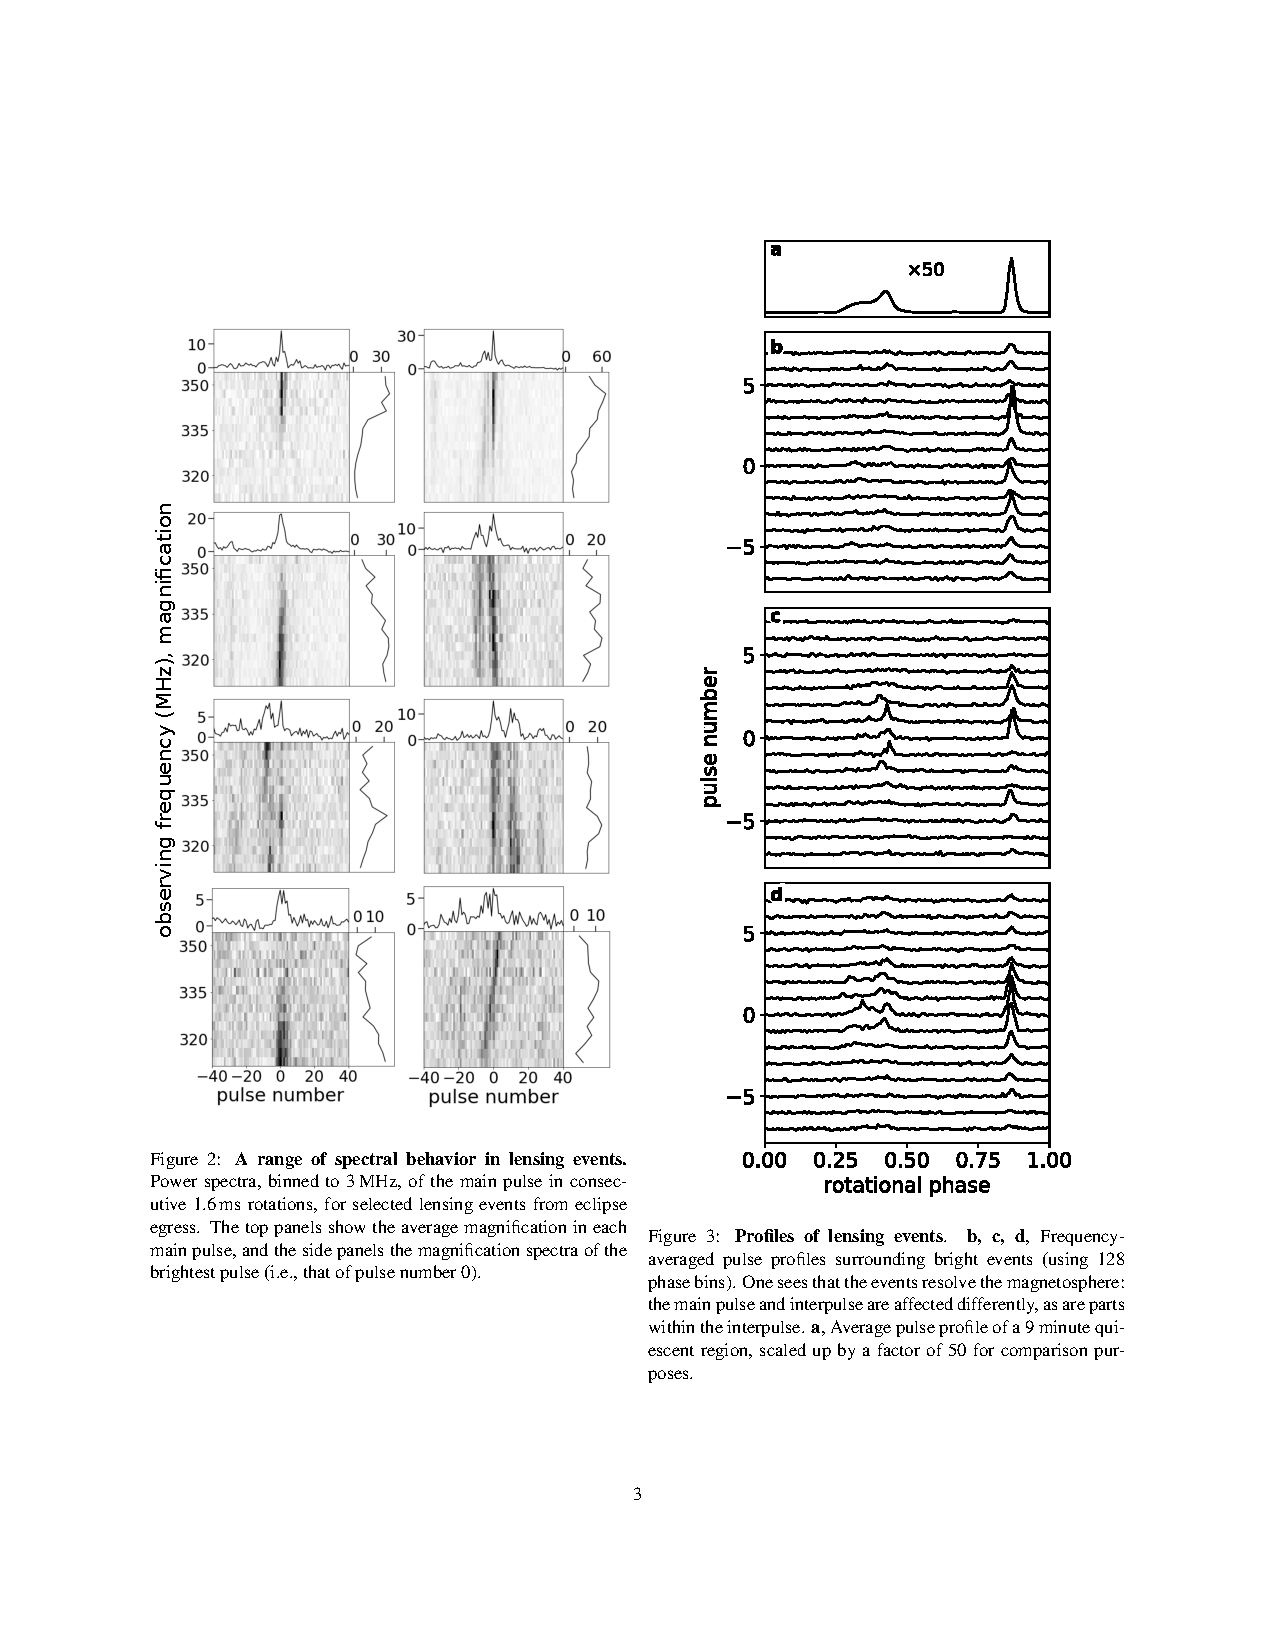
\includegraphics[width=0.75\textwidth]{Figures/bwlens.pdf}

     Main++ULP2018, Nature,  557, 522
}


\frame{
    \frametitle{BURSTT}
Bustling Universe Radio Telescope Taiwan: collaboration of ASIAA, NTU,
NTHU, NCHU for all sky FRB radio array
     \hspace{-0.5in}
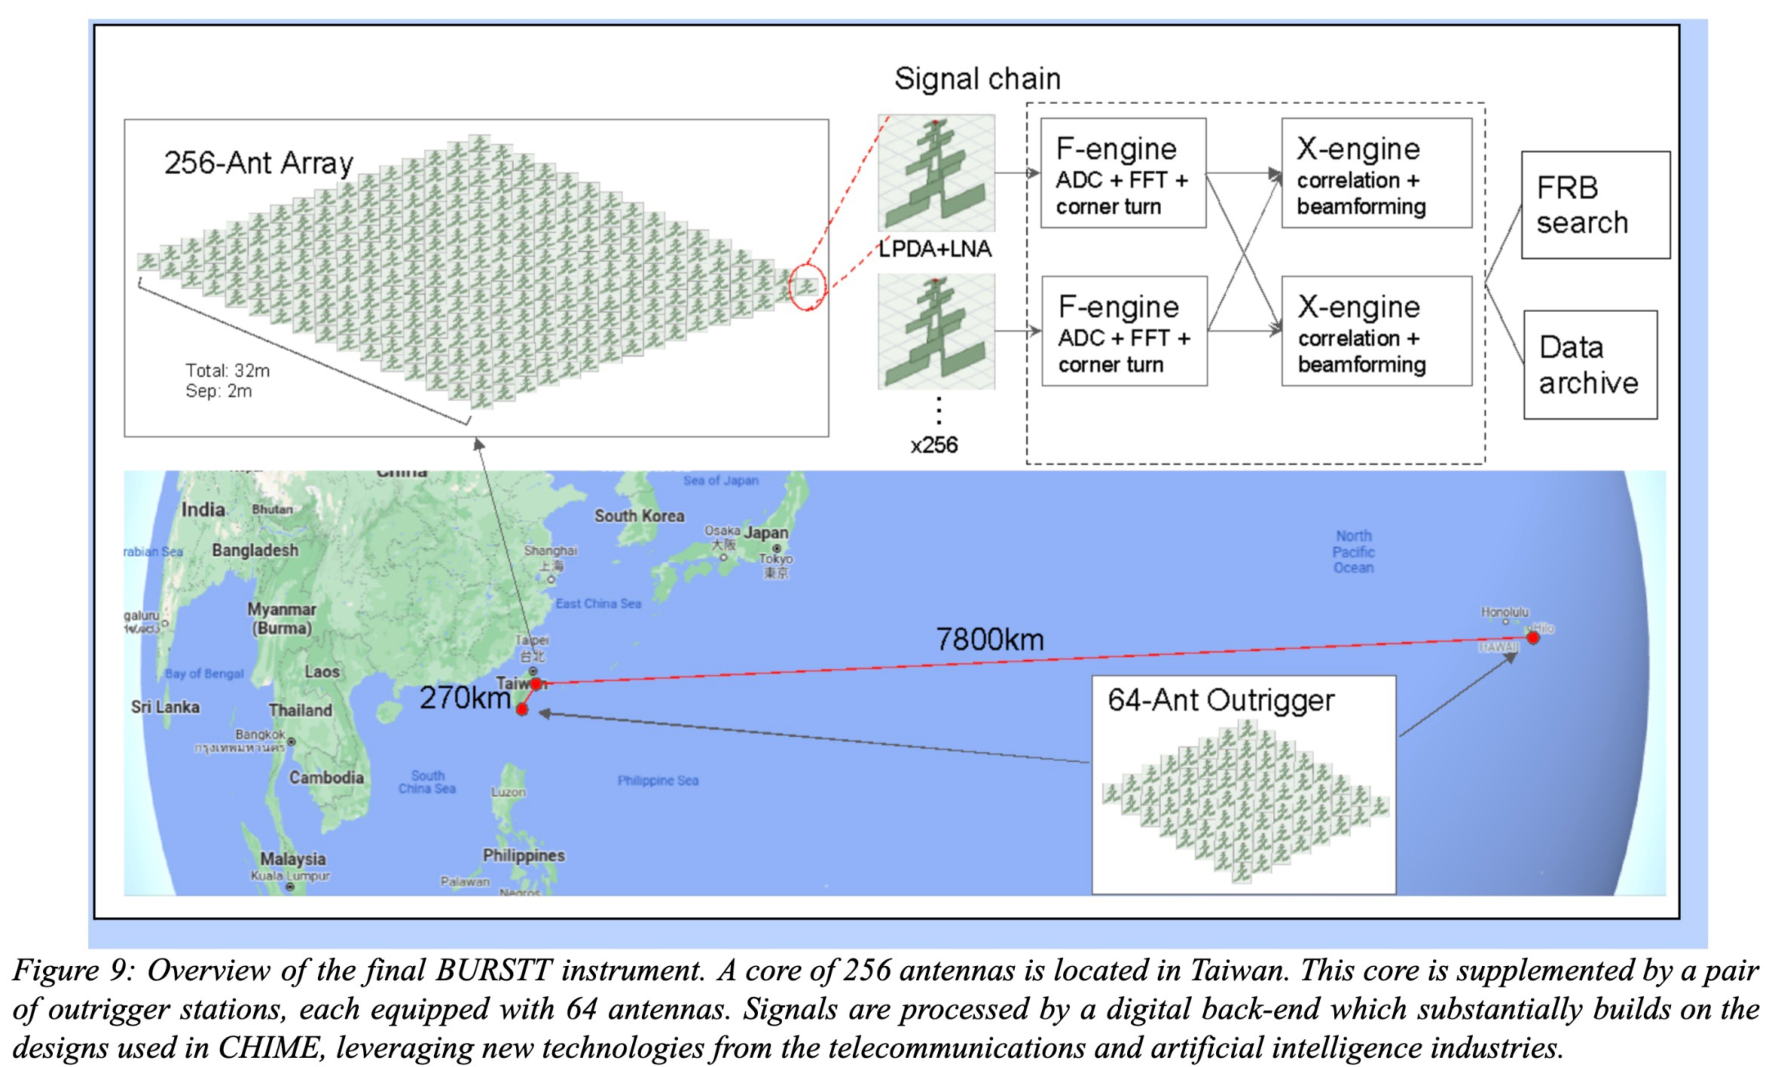
\includegraphics[width=0.55\textwidth]{Figures/BURSTT.pdf}
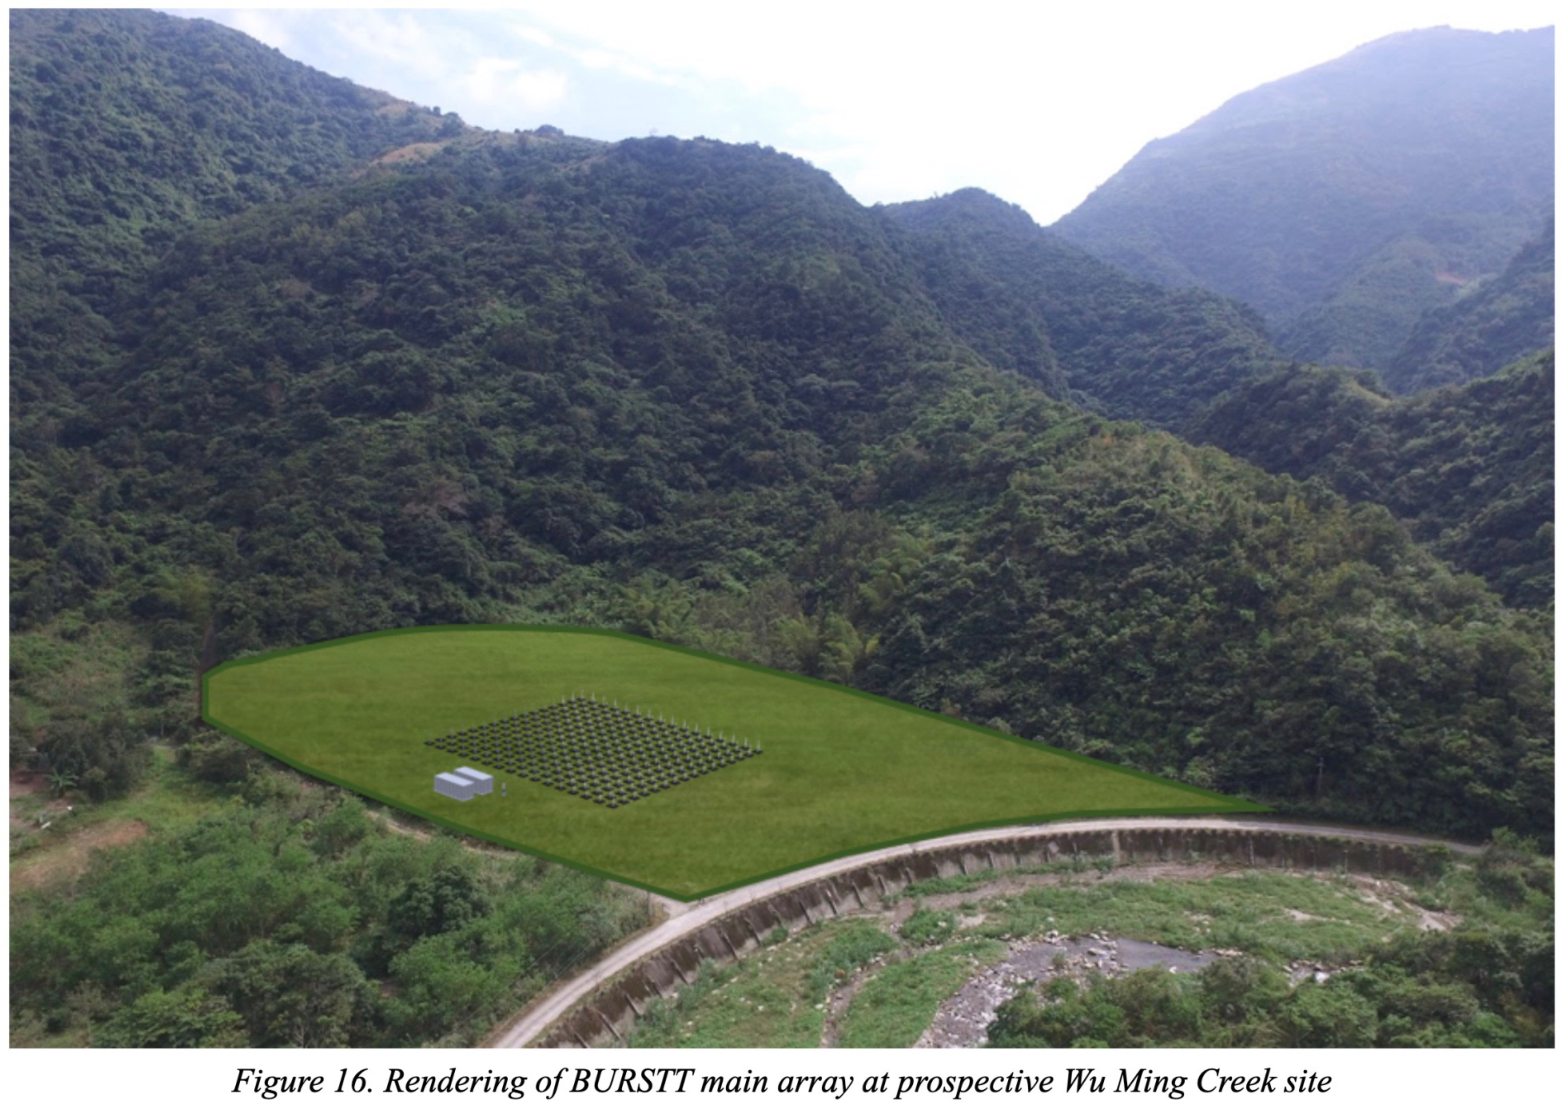
\includegraphics[width=0.45\textwidth]{Figures/BURSTTN.pdf}


}


  \frame{
\vspace{-0.5in}
    \frametitle{Conclusions}
    \begin{itemize}
    \item wave optics changes nature of astrophysical observables: Coherent FRB
      radiation one of the potentially most
      precise measurements in physics
    \item coherent radio waves (FRBs, pulsars): described by Eikonal
      away from caustics/catastrophies
    \item long wavelength GW (FRB microlensing, LIGO, LISA, PTA): full wave effects, P-L theory
    \item importance of imaginary images
    \end{itemize}
  }

\end{document}
